%!TEX root = Memoria_TFM.tex
\section{Metrics}
To characterize a system, it is necessary metrics that evaluate it. In this section the used metrics along the thesis are exposed.\\

Before describing the parameters it is necessary define that the posed problem is bi-class, that means that only two classes would be used:
\begin{description}[itemsep=2pt,topsep=8pt,parsep=0pt,partopsep=20pt]
\item \textbf{Positive class}: are the samples of the real users, the genuine or \textit{bona fide}.
\item \textbf{Negative class}: are the different attacks samples which that pretend to be real users but not.
\end{description}

\subsection{Cost and Error rate}
The first parameter that is used is the cost. The cost is used while the neural network is training, in fact, is the value that must be minimized during the training. The lower value, The better performance of the network.\\

The cost calculated with the Minibatch Stochastic Gradient Descent (MSGD) is the Negative Log-Likelihood Loss. The MSGD is a variant of the Stochastic Gradient Descent in which the cost is calculated with a mini batch of data, not each sample independently and the Loss is the accumulation \cite{Stutz}.\\

The loss is calculated in the following way:\\

\begin{equation}
  Loss(\theta, D) = - \sum_{i=0}^{|D|}log P(Y = y^{(i)}|x^{(i)}, \theta)
\end{equation}

The error in the validation process is calculated after the logistic regression classification, because is the classifier used during the training process. The error during the testing procedure depends on the used classifier. In both cases, the error represents the number of misclassified samples over the total samples used.

\subsection{True Positives (TP), True Negatives (TN), False Positives (FP), False Negatives (FN)}
If each predicted class is compared with it real target, True Positives (TP), True Negatives (TN), False Positives (FP), False Negatives (FN) values could be calculated. These metrics are usually used for bi-classes problems.\\

Those metrics, are gotten when positive or negative samples are correctly or incorrectly classified \cite{Sokolova}. The classified or predicted sample is compared with its real target.\\

If a positive sample is classified as positive is a true positive (TP), but if it has been classified as negative is a false negative (FN).\\

If a negative sample is classified as negative is a true negative (TN), but if it has been classified as positive, is a false positive (FP).\\

From those four metrics, it could be extracted the confusion matrix for binary classification which is defined in table \ref{table:ConfusionMatrix} \cite{ROC, Sokolova}:

\begin{table}[htb]
\centering
\begin{tabular}{|
>{\columncolor[HTML]{ECF4FF}}c |>{\columncolor[HTML]{FFFFFF}}c | >{\columncolor[HTML]{FFFFFF}}c |}
\hline
\textbf{Real / Classified} & \cellcolor[HTML]{ECF4FF}\textbf{Positive} & \cellcolor[HTML]{ECF4FF}\textbf{Negative} \\ \hline
\textbf{Positve}           & TP                                        & FN                                        \\ \hline
\textbf{Negative}          & FP                                        & TN                                        \\ \hline
\end{tabular}
\caption{Confusion Matrix.} \label{table:ConfusionMatrix}
\end{table}

The confusion Matrix resume these four metrics in a table. Both, the confusion matrix or the parameters individually, are widely utilized.

\subsection{ROC curve and Equal Error Rate (EER)}
From the confusion matrix, it is possible calculate others parameters \cite{Sokolova}: precision, recall, specificity, accuracy, etc. because its values depend on TP, TN, FP, FN:
\begin{itemize}
\item The False Positive Rate (FPR) is defined as the proportion of all the negative samples (\textit{N}) that are classified as positive incorrectly \cite{ROC}:

\begin{equation}
FPR = \frac{FP}{N}
\end{equation}
Where:
 \begin{equation}
  N = FP + TN
\end{equation}

\item The True Positive Rate (TPR) is defined as the proportion of all the positive samples (\textit{P}) that are classified correctly \cite{ROC}. This parameter could be known as Recall too:
\begin{equation}
TPR = Recall = \frac{TP}{P}
\end{equation}
Where:
 \begin{equation}
  P = TP + FN
\end{equation}
%TPR could be called sensitivity and FPR could be calculated as 1 – specificity \\
\item False Acceptance Rate (FAR): is defined as the incorrectly accepted users with respect all the samples.
\begin{equation}
  FAR = \frac{FP}{P + N}
\end{equation}

\item False Rejection Rate (FRR): is defined as the incorrectly rejected users with respect all the samples.
\begin{equation}
  FRR = \frac{FN}{P + N}
\end{equation}

%\item Precision is defined as the proportion of real positive samples that has been classified as positive \cite{ROC,Sokolova}:
%\begin{equation}
 % precision = \frac{TP}{TP + FP}
%\end{equation}

\item Accuracy is defined as the proportion of the correctly classified samples of all the samples \cite{Sokolova}. The classifiers implemented in scikit-learn library return this value as metric.:
\begin{equation}
  Accuracy = \frac{TP + TN}{TP + FP + FN + TN}
\end{equation}
\end{itemize}

The Receiver Operator Characteristic (ROC) curve is the representation how the number of positives samples, which has been classified correctly, changes with the number of negative samples incorrectly classified. The ROC curve is defined by the parameters False Positive Rate (FPR) and True Positive Rate (TPR) \cite{ROC}.\\

\begin{figure}[htb]
  \centering
  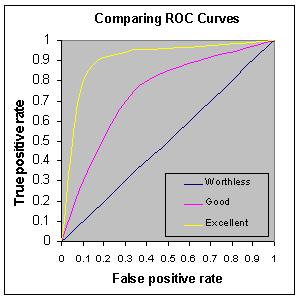
\includegraphics[width=0.4\textwidth]{images_miscelaneus/roccomp.jpg}
  \caption{ROC curves. Image obtained from \cite{RocImage}.}
  \label{RocImage}
\end{figure}

The figure \ref{RocImage}, obtained from \cite{RocImage}, demonstrates a ROC graph in which three curves are portrayed.  The yellow one represents a good classification, it is the desired ROC curve, but the blue curve represents a bad classification and it is not the desired result.\\

From the ROC curve, the Area Under the Curve (AUC) could be obtained, this value is the integral of the ROC curve, and its maximum value is 1 that means a perfect performance of the classifier. If the value of this parameter is lower than 0.7 the classifier performance required to be improved significantly.\\

From FAR and FRR rates it is possible to calculate the Equal Error Rate (ERR) and it is obtained at the point where FAR and FRR acquire the same value. The closest is its value to 0, the better is the performance of the classifier.

%The Precision and Recall curve is the representation of the Precision and the Recall in the same graph. The desired behaviour of a classification system is a high recall (1) and a high precision (1) because that would mean that predictions made by the classifier are correct.\\

\subsection{APCER and BPCER}
The ISO/IEC 30107-3 \cite{ISO} is the collaboration result of  the International Organization for Standardization (ISO) with the International Electrotechnical Commission (IEC).\\

The ISO defines the terms related to the tests, the reports and the biometric presentation of biometrics systems. In addition, the performance methods, specify principles as well as metrics are defined. From this document, the APCER, BPCER and APCER-BPCER curve metrics have been obtained:\\

Attack Presentation Classification Error Rate (APCER) is defined as the proportion of presentation attacks that has been classified incorrectly (as \textit{bona fide} presentation.)\\

\begin{equation}
  APCER_{PAIS} = \frac{1}{N_{PAIS}}\sum_{i=1}^{N_{PAIS}}(1 - Res_{i})
\end{equation}

\textit{Bona fide} Presentation Classification Error Rate (BPCER) is defined as the proportion of \textit{bona fide} presentations  incorrectly classified as presentation attacks.\\

\begin{equation}
  BPCER = \frac{\sum_{i=1}^{N_{BF}}Res_{i}}{N_{BF}}
\end{equation}

where: \begin{itemize}
\item $N_{BF}$ is the number of \textit{bona fide} presentations
\item $Res_{i}$ is 1 if $i^{th}$ presentation is classified as an attack and 0 if is classified as a \textit{bona fie} presentation.
\item $N_{PAIS}$ is the number of attack presentations
\end{itemize}

The APCER-BPCER curve illustrates in the same graph both parameters. The ideal system would have a low APCER (0) and a low BPCER (0) because it means that samples are not incorrectly classified.
